\documentclass{article}
\usepackage[utf8]{inputenc}
\usepackage{geometry}
\usepackage{graphicx}
\usepackage{amsmath}
\usepackage{amsfonts}
\usepackage{amsthm}
\usepackage{amssymb}
\usepackage[most]{tcolorbox}
\usepackage{array}
\usepackage{latexsym}
\usepackage{alltt}
\usepackage{hyperref}
\usepackage{color, colortbl}
\usepackage{float}
\usepackage{pdfpages}
\usepackage{algpseudocode}
\usepackage{multicol}
\usepackage{multirow}
\usepackage{caption}
\usepackage{xparse}
\usepackage{setspace}
\usepackage{enumitem}
\usepackage{pdflscape}
% \usepackage{parskip}
\usepackage{blindtext}
\usepackage{forest}
% \usepackage[newfloat]{minted}
\usepackage{booktabs}


\geometry
{
  a4paper,
  left=12mm,
  right=12mm,
  top=12mm,
  bottom=15mm,
}

% mybox
\newtcolorbox{mybox}[3][]
{
  colframe = #2!25,
  colback  = #2!10,
  coltitle = #2!20!black,  
  title    = {#3},
  #1,
}

\definecolor{ex}{rgb}{1.00,0.65,0.00}
\definecolor{bg}{rgb}{0.95,0.95,0.95}
% \setminted
% {
% 	mathescape=true,
% 	xleftmargin=\parindent,
% 	bgcolor=bg,
% 	escapeinside=@@
% }

% \SetupFloatingEnvironment{listing}{name=Code}

% New environments that use mybox
\newcounter{example}[section]
\newenvironment{example}[1]{\begin{mybox}[breakable]{ex}{\refstepcounter{example}\textbf{Example \thesection.\theexample #1}}}{\end{mybox}}

\newcounter{definition}[section]
\newenvironment{definition}[1]{\refstepcounter{definition}\begin{mybox}[breakable]{blue}{\textbf{Definition \thesection.\thedefinition #1}}}{\end{mybox}}

\newcounter{theorem}[section]
\newenvironment{theorem}[1]{\begin{mybox}{red}{\refstepcounter{theorem}\textbf{Theorem \thesection.\thetheorem #1}}}{\end{mybox}}

\newenvironment{formula}[1]{\begin{mybox}{cyan}{\textbf{#1}}}{\end{mybox}}

\newenvironment{practice}[1]{\begin{mybox}{ex}{\textbf{#1}}}{\end{mybox}}

% Changing maketitle
\makeatletter         
\renewcommand\maketitle{
{\raggedright % Note the extra {
\begin{center}
{\Large \bfseries \@title}\\[2ex] 
{\large \@author \ - \@date}\\[2ex]
\end{center}}} % Note the extra }
\makeatother

% \onehalfspacing % adjust spacing
\setlength{\parskip}{0.5\baselineskip}

% macros
\newcommand{\prob}[1]{\textbf{\textit{P}}\left\{#1\right\}}
\newcommand{\expc}[1]{\mathbf{E}\left(#1\right)}
\newcommand{\expcs}[1]{\mathbf{E}^2\left(#1\right)}
\newcommand{\var}[1]{\text{Var}\left( #1 \right)}
\newcommand{\ra}{\rightarrow}
\newcommand{\Ra}{\Rightarrow}
\newcommand{\R}[2]{\tikz [remember picture,overlay] \node (#1) {#2};}

\def\circtxt#1{$\mathalpha \bigcirc \mkern-13mu \mathtt #1$}
\def\smiley{\textcircled{\scriptsize $\mkern3mu\ddot{\ } \mkern-15mu \smallsmile$}}

\NewDocumentCommand{\dsum}{%
    e{^_}
}{%
  {% 
    \displaystyle\sum
    \IfValueT{#1}{^{#1}}
    \IfValueT{#2}{_{#2}}
  }
}%

% maketitle variables
\title{CENG 232 - Chapter 6: Registers and Counters}
\author{Burak Metehan Tunçel}
\date{May 2022}

\begin{document}

\maketitle

\begin{multicols*}{2}
\setlength{\columnsep}{1.5cm}
\setlength{\columnseprule}{0.2pt}

\section{Registers}
\label{sec:registers}

\begin{itemize}[leftmargin=0.7cm]
  \item A \textbf{register} is a \textit{group of flip-flops}, each one of which shares a common clock and is capable of storing one bit of information. An $n$-bit register consists of a group of $n$ flip-flops capable of storing $n$ bits of binary information. In addition to the flip-flops, a register may have combinational gates that perform certain data-processing tasks. 

  In its broadest definition, a register consists of a group of flip-flops together with gates that affect their operation. The flip-flops hold the binary information, and the gates determine how the information is transferred into the register.

  \item A \textbf{counter} is essentially \textit{a register that goes through a predetermined sequence of binary states}. The gates in the counter are connected in such a way as to produce the prescribed sequence of states. Although counters are a special type of register, it is common to differentiate them by giving them a different name.
\end{itemize}

\noindent The simplest register is one that consists of only flip-flops, without any gates. Figure 1 shows such a register constructed with four $D$-type flip-flops to form a four-bit data storage register.


\subsection{Register with Parallel Load}
\label{subsec:register-with-parallel-load}

The transfer of new information into a register is referred to as \textit{loading} or \textit{updating} the register. If all the bits of the register are loaded simultaneously with a common clock pulse, we say that the loading is done in \textit{parallel}.

If the contents of the register must be left unchanged, the inputs must be held constant or the clock must be inhibited from the circuit.
\begin{itemize}[leftmargin=0.7cm]
  \item In the first case, the data bus driving the register would be unavailable for other traffic.
  \item In the second case, the clock can be inhibited from reaching the register by controlling the clock input signal with an enabling gate.
\end{itemize}

The solution can be implementing the additional gates in either the data bus or the output of the register to allow data to load or update. In Fig. 2, load input is implemented.

\vspace*{\fill}
\columnbreak

\begin{figure}[H]
  \centering
  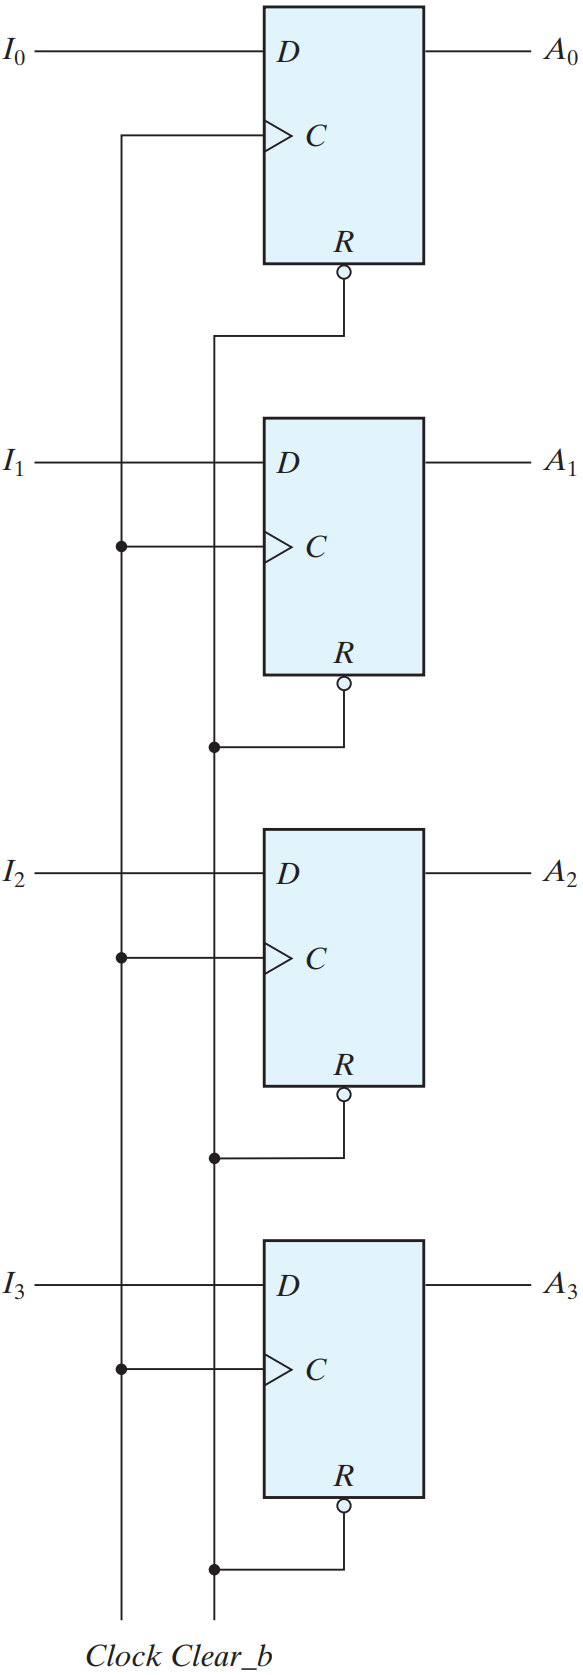
\includegraphics[width=.9\linewidth]{img/fig-6.1.png}
  \caption{Four-bit register}
  \label{fig:6.1}
\end{figure}

\begin{figure}[H]
  \centering
  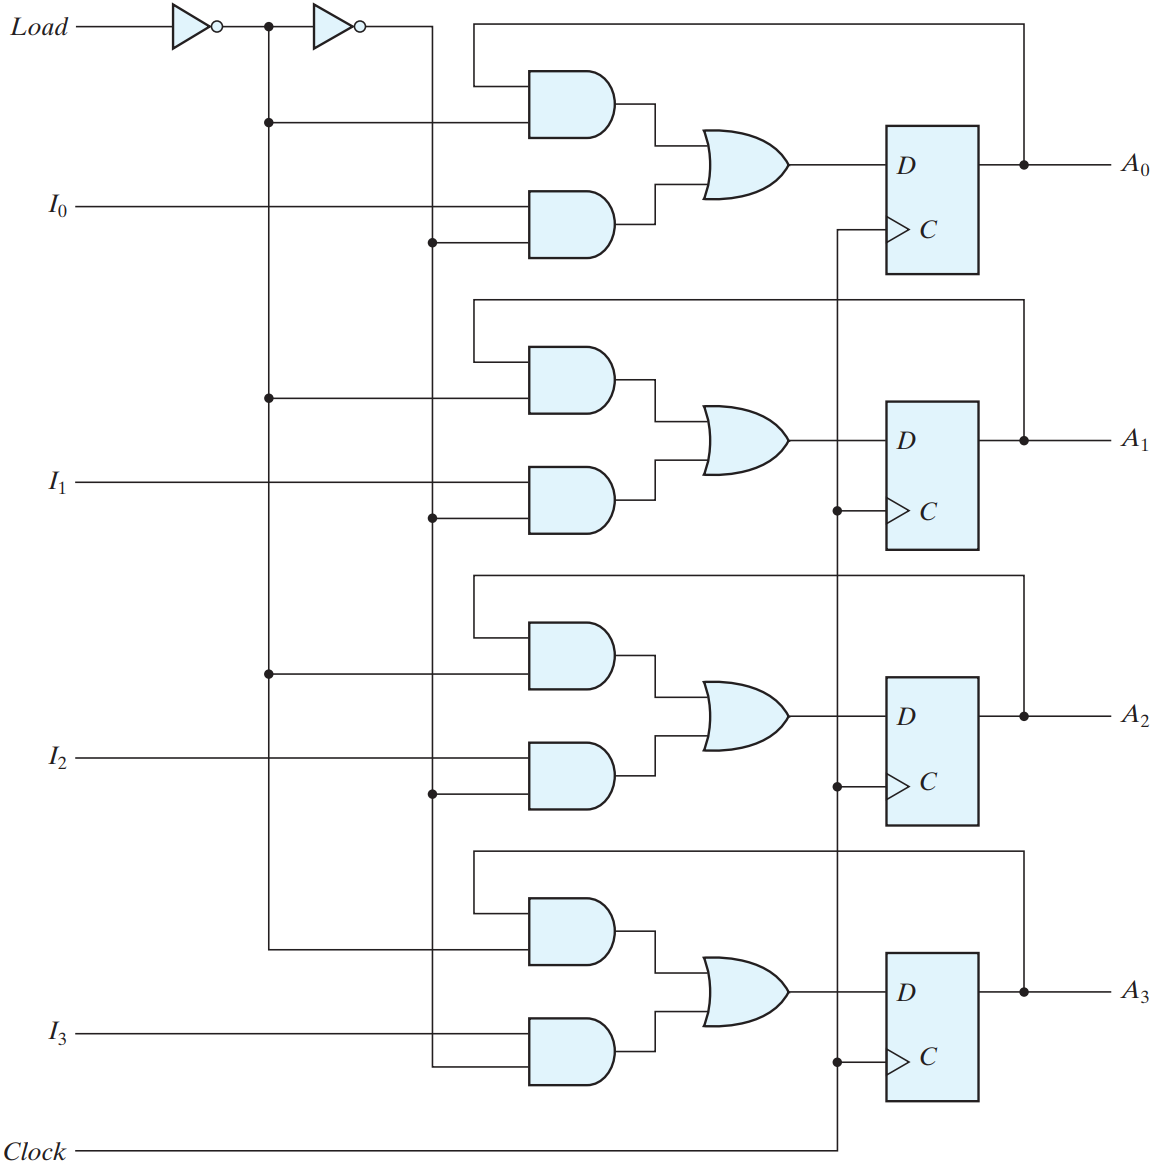
\includegraphics[width=\linewidth]{img/fig-6.2.png}
  \caption{Four-bit register with parallel load}
  \label{fig:6.2}
\end{figure}


\section{Shift Registers}
\label{sec:shift-registers}

A register capable of shifting the binary information held in each cell to its neighboring cell, in a selected direction, is called a \textit{shift register}.
The simplest possible shift register is one that uses only flip-flops, as shown in Fig. 3.
\begin{figure}[H]
  \centering
  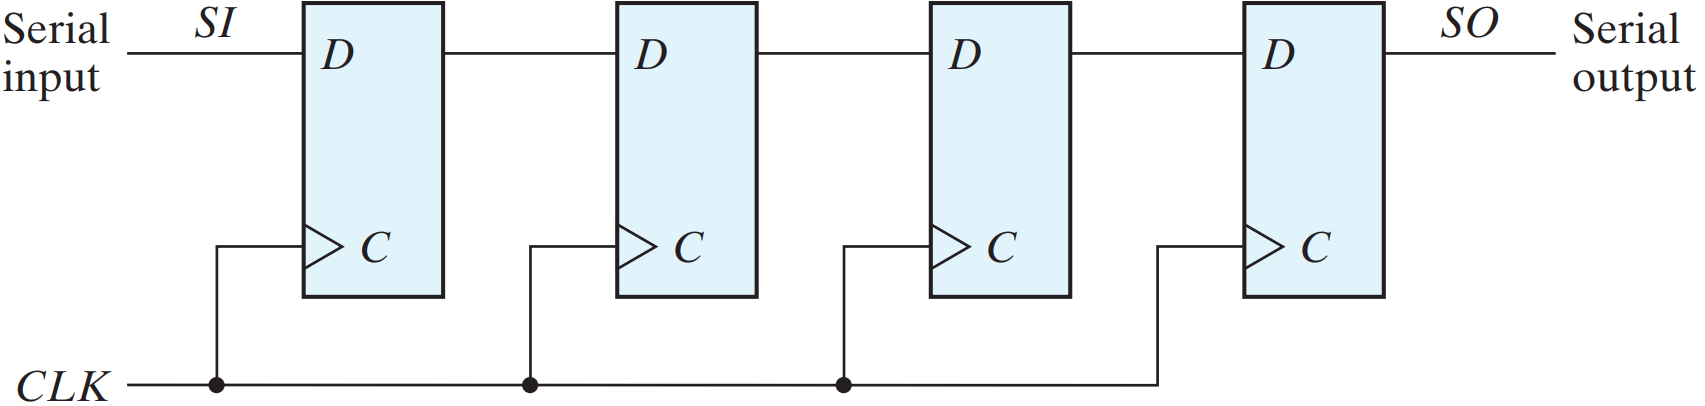
\includegraphics[width=\linewidth]{img/fig-6.3.png}
  \caption{Four-bit shift register}
  \label{fig:6.3}
\end{figure}
\noindent This shift register is unidirectional (left-to-right). Each clock pulse shifts the contents of the register one bit position to the right.

\subsection{Serial Transfer}
\label{subsec:serial-transfer}

The datapath of a digital system is said to operate in serial mode when \textit{information is transferred and manipulated one bit at a time}. The serial transfer of information from register $A$ to register $B$ is done with shift registers, as shown in the block diagram of Fig. 6.4(a).
\begin{figure}[H]
  \centering
  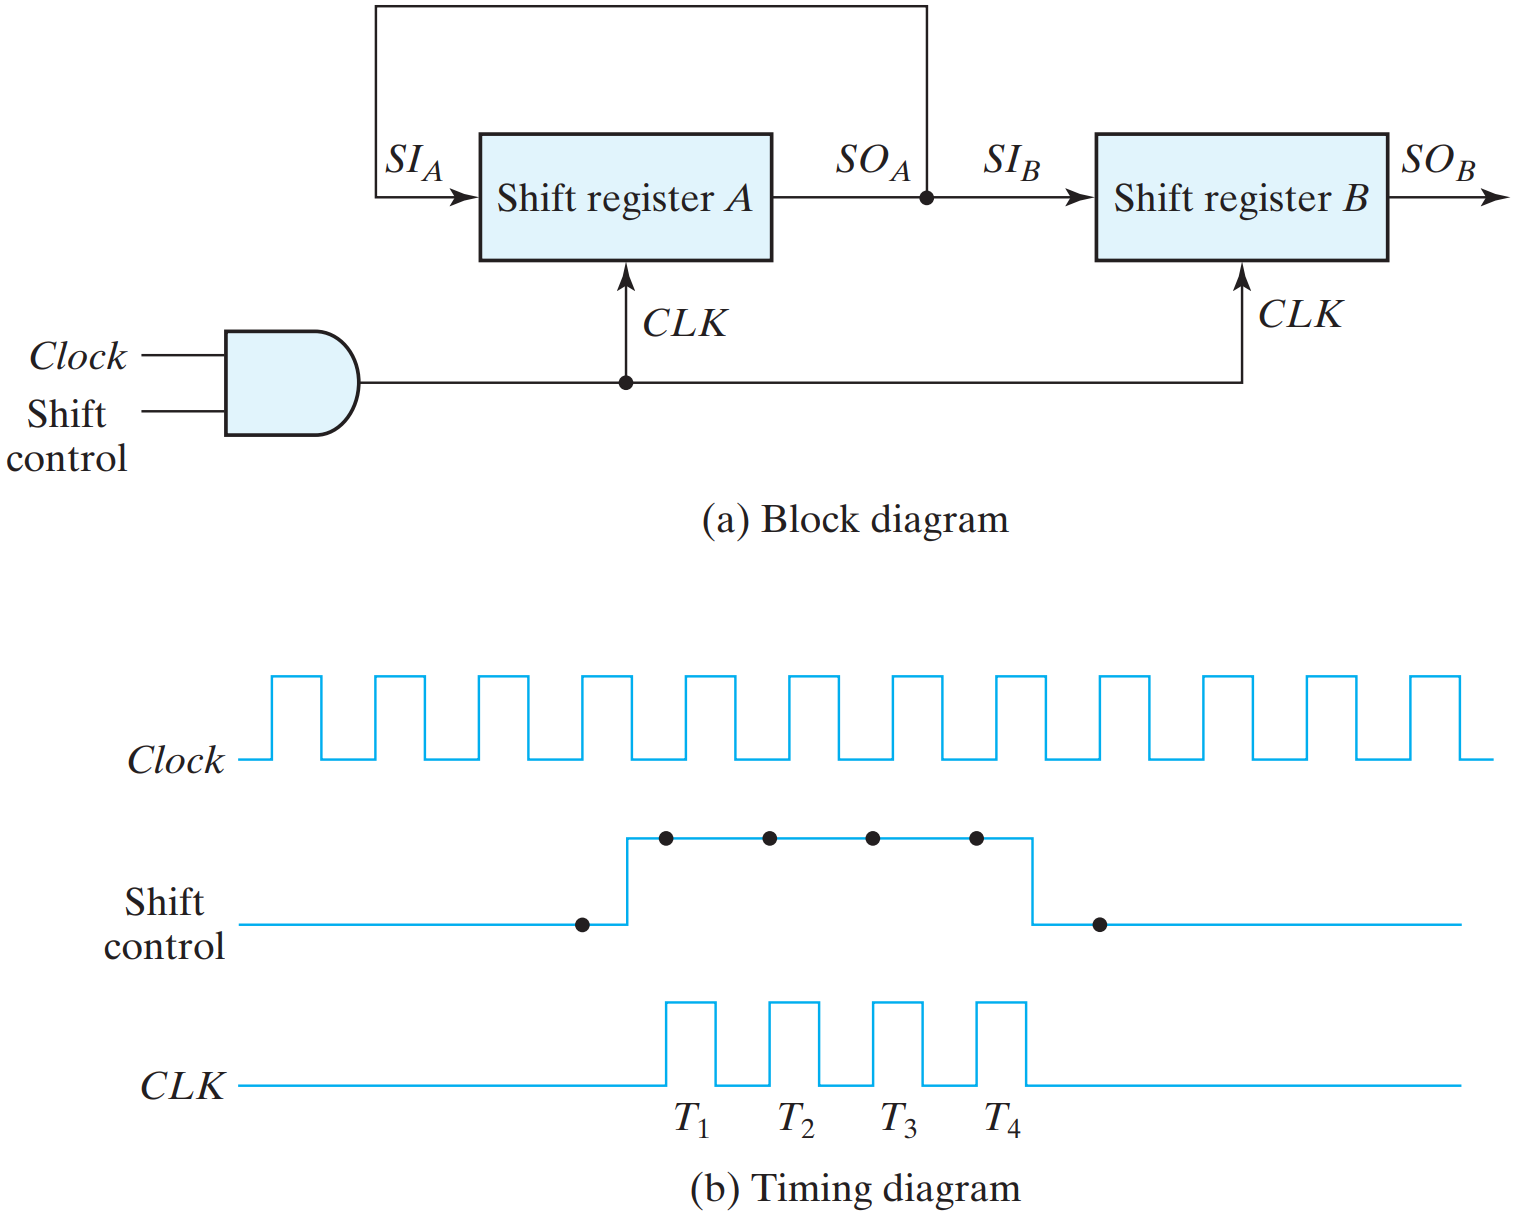
\includegraphics[width=\linewidth]{img/fig-6.4.png}
  \caption{Serial transfer from register $A$ to register $B$}
  \label{fig:6.4}
\end{figure}
\noindent Four pulses: $T_1$, $T_2$, $T_3$, and $T_4$. Each rising edge of the pulse causes a shift in both registers.
\begin{figure}[H]
  \centering
  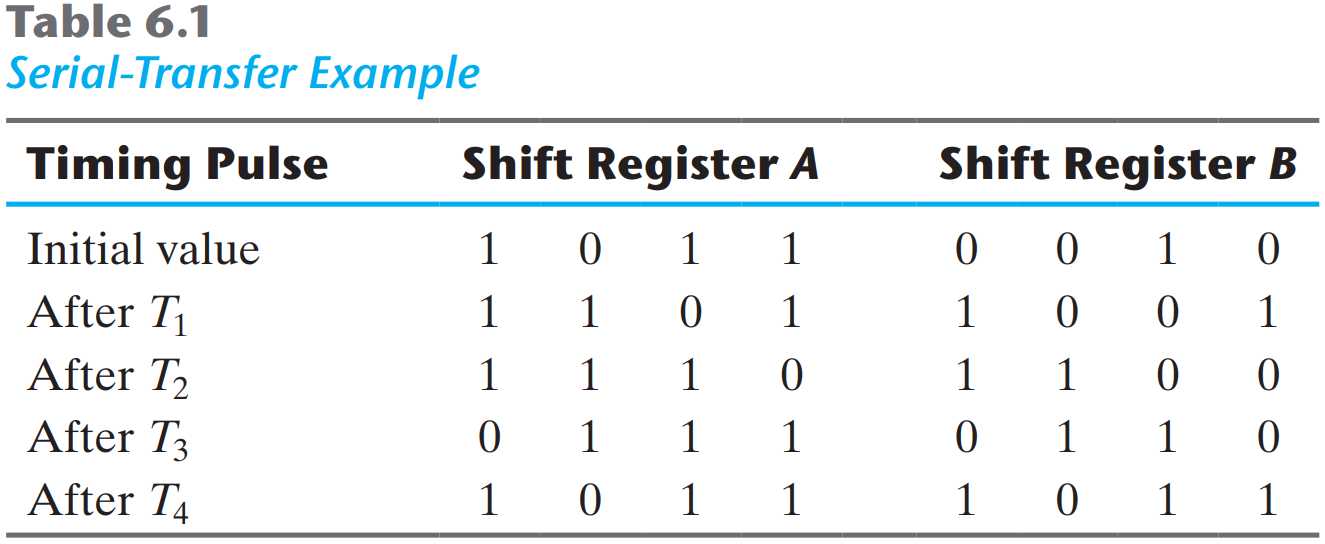
\includegraphics[width=\linewidth]{img/table-6.1.png}
  \label{table:6.1}
\end{figure}

One application of shift registers is converting between ``serial data'' and ``parallel data''. Computers typically work with multiple-bit quantities (ASCII: 8 bits long; Integers: 32 bits long.). But sometimes it's necessary to send or receive data serially, or one bit at a time. Some examples includes: Input devices such as keyboards and mice or output devices like printers.

\noindent Receiving serial data:
\begin{figure}[H]
  \centering
  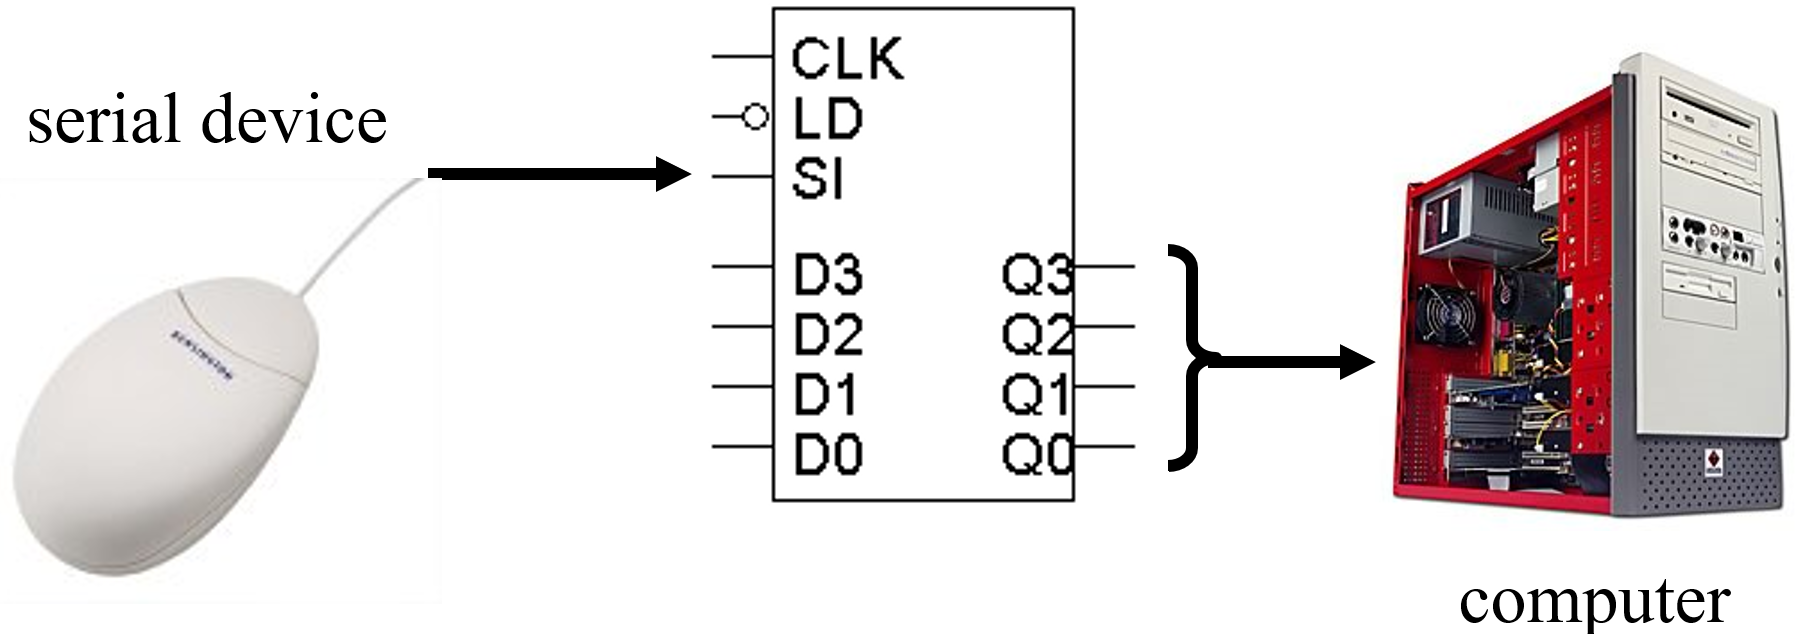
\includegraphics[width=\linewidth]{img/receiving-serial-data.png}
\end{figure}
\noindent Sending data serially:
\begin{figure}[H]
  \centering
  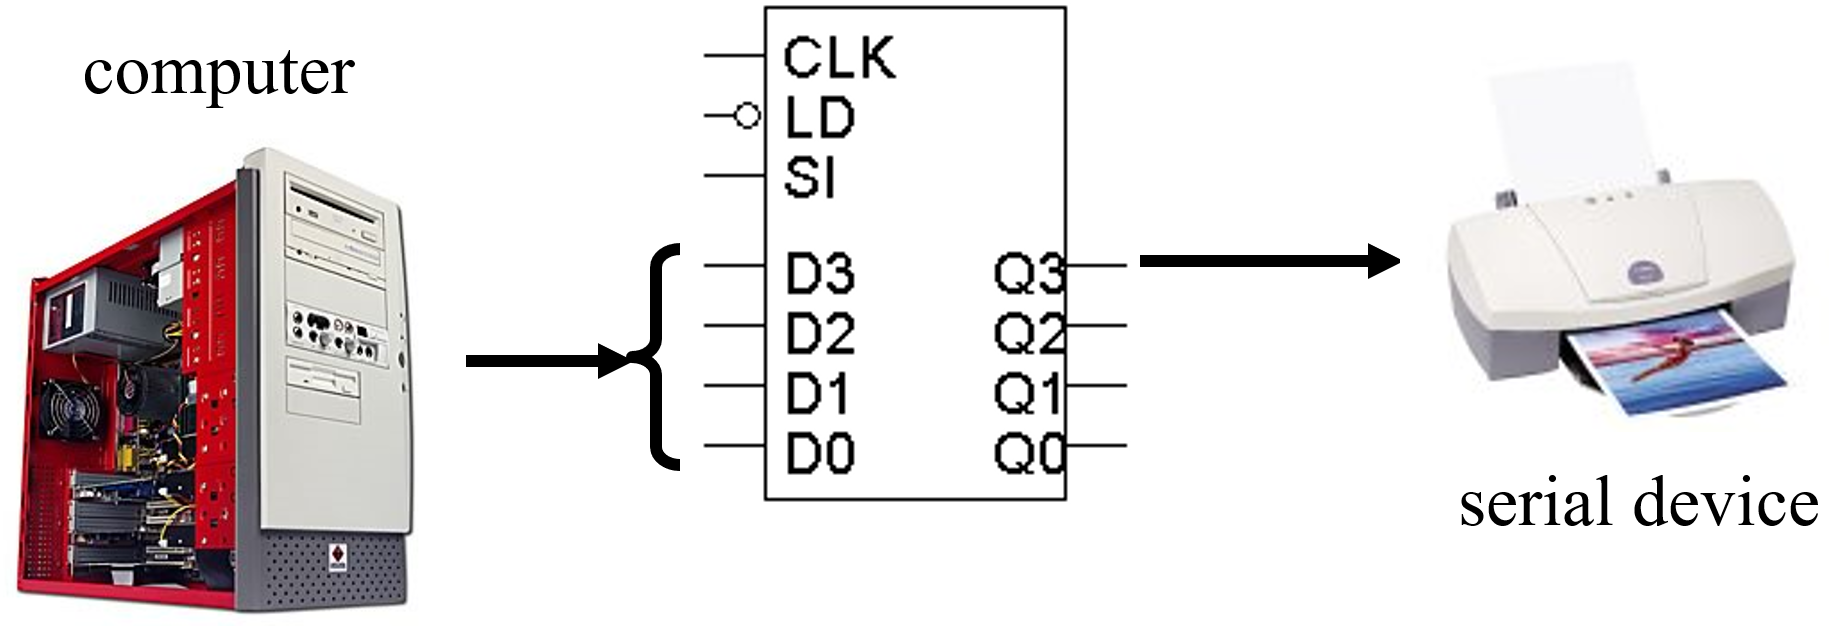
\includegraphics[width=\linewidth]{img/sending-data-serially.png}
\end{figure}

\subsection{Serial Addition}
\label{subsec:serial-addition}

The two binary numbers to be added serially are stored in two shift registers. Beginning with the least significant pair of bits, the circuit adds one pair at a time through a single full-adder (FA) circuit, as shown in Fig. 5.
\begin{figure}[H]
  \centering
  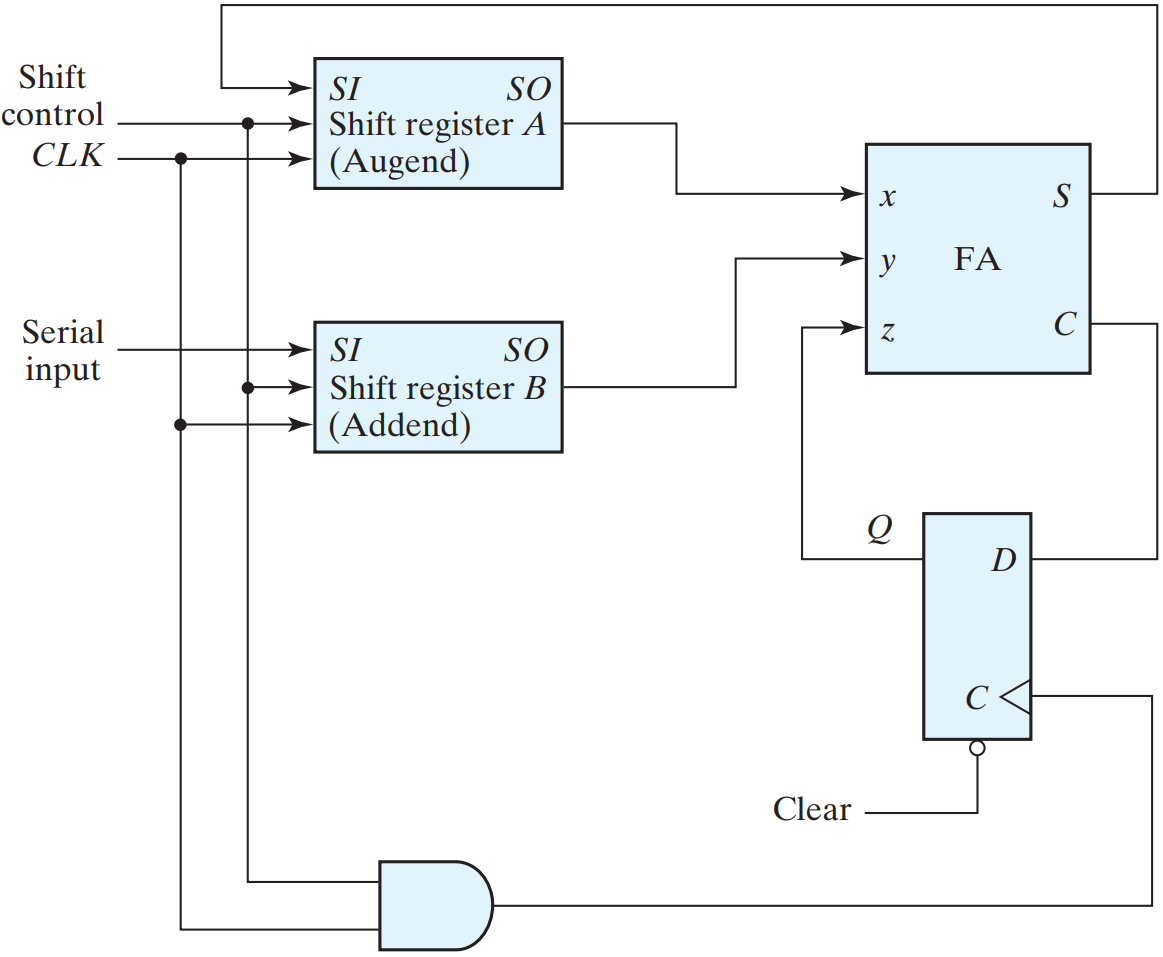
\includegraphics[width=\linewidth]{img/fig-6.5.png}
  \caption{Serial adder}
  \label{fig:6.5}
\end{figure}
Comparing the serial adder with the parallel adder, we note several differences.
\begin{itemize}
  \item The parallel adder uses registers with a parallel load, whereas the serial adder uses shift registers.
  \item The number of full-adder circuits in the parallel adder is equal to the number of bits in the binary numbers, whereas the serial adder requires only one full-adder circuit and a carry flip-flop.
  \item Excluding the registers, the parallel adder is a combinational circuit, whereas the serial adder is a sequential circuit, which consists of a full adder and a flip-flop that stores the output carry.
\end{itemize}

\noindent \textbf{Serial Adder with JK Flip-Flop:}
\begin{figure}[H]
  \centering
  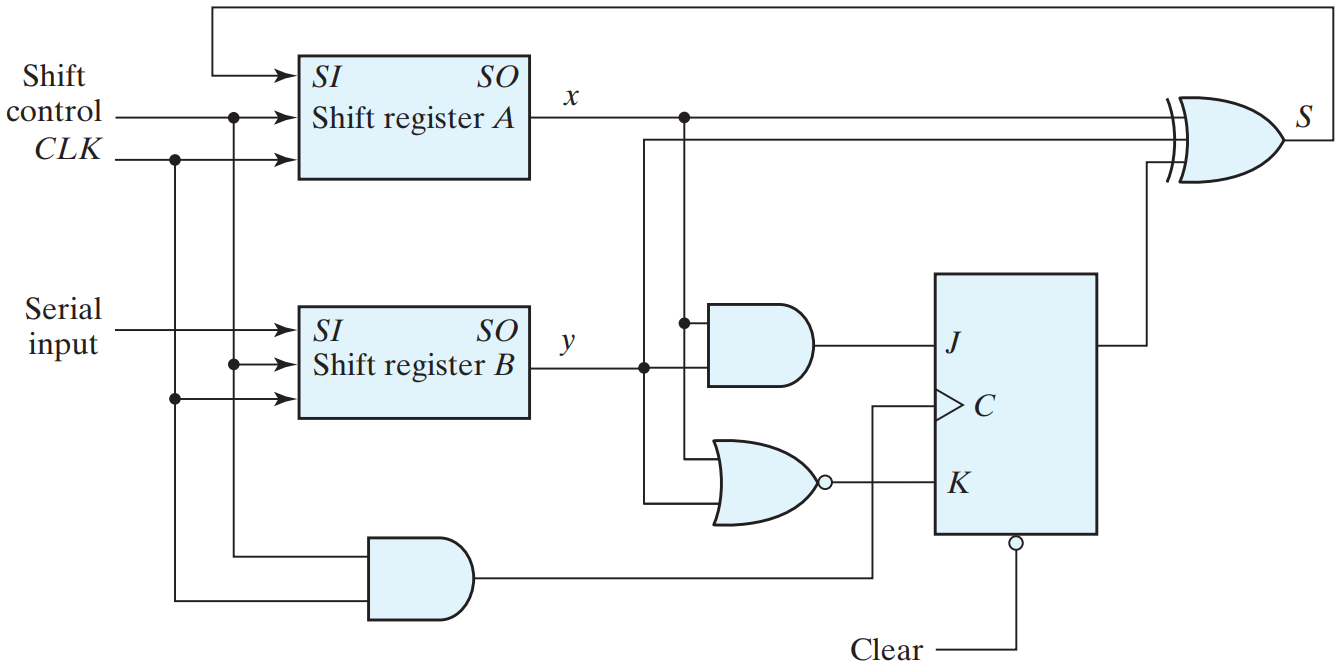
\includegraphics[width=\linewidth]{img/fig-6.6.png}
  \caption{Serial adder}
  \label{fig:6.6}
\end{figure}

\vspace*{\fill}
\columnbreak

\subsection{Universal Shift Register}
\label{subsec:universal-shift-register}

Some shift registers provide the necessary input and output terminals for parallel transfer. They may also have both shift-right and shift-left capabilities. The most general shift register has the following capabilities:
\begin{enumerate}[leftmargin=0.7cm]
  \item A \textit{clear} control to clear the register to 0.
  \item A \textit{clock} input to synchronize the operations.
  \item A \textit{shift-right} control to enable the shift-right operation and the \textit{serial input} and \textit{output lines} associated with the shift right.
  \item A \textit{shift-left} control to enable the shift-left operation and the \textit{serial input} and \textit{output lines} associated with the shift left.
  \item A \textit{parallel-load} control to enable a parallel transfer and the $n$ input lines associated with the parallel transfer.
  \item $n$ parallel output lines.
  \item A control state that leaves the information in the register unchanged in response to the clock.
\end{enumerate}

If the register can shift in both directions and has parallel-load capabilities, it is referred to as a \textit{universal shift register}.

The block diagram symbol and the circuit diagram of a four-bit universal shift register that has all the capabilities just listed are shown in Fig. 7. The circuit consists of four $D$ flip-flops and four multiplexers. The four multiplexers have two common selection inputs $s_1$ and $s_0$.

\begin{figure}[H]
  \centering
  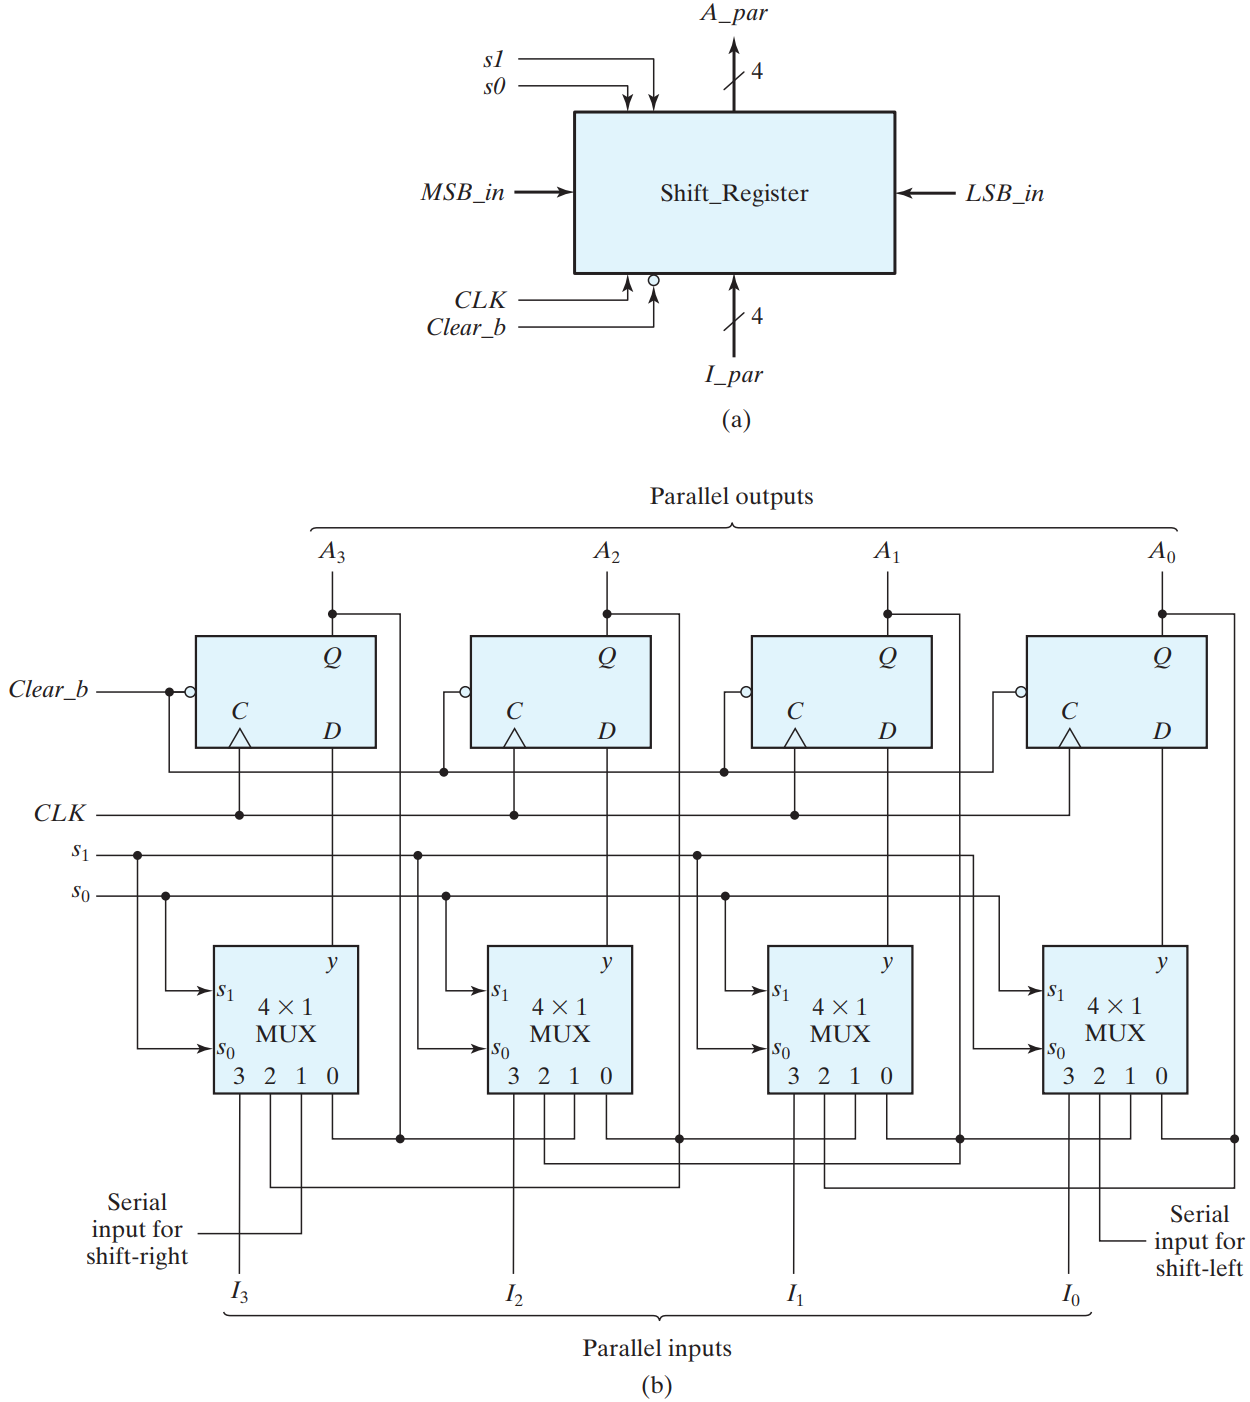
\includegraphics[width=\linewidth]{img/fig-6.7.png}
  \caption{Four-bit universal shift register}
  \label{fig:6.7}
\end{figure}

\vspace*{\fill}
\columnbreak

\begin{figure}[H]
  \centering
  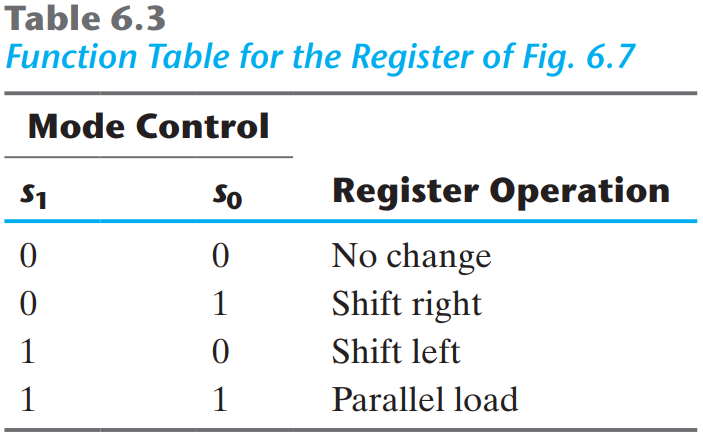
\includegraphics[width=\linewidth]{img/table-6.3.png}
  \label{table:6.3}
\end{figure}

\noindent\rule{\linewidth}{1pt}

\begin{figure}[H]
  \centering
  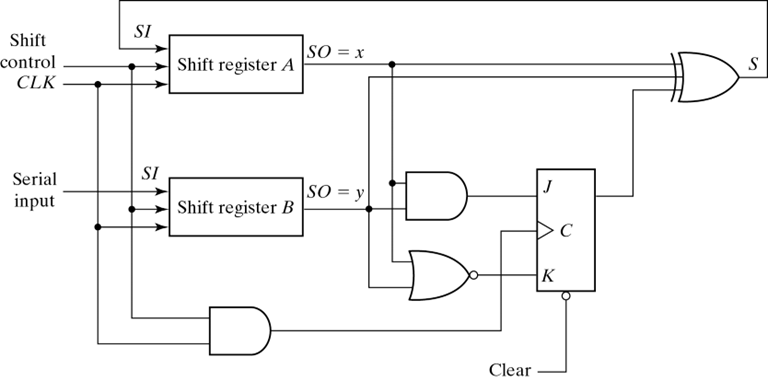
\includegraphics[width=\linewidth]{img/serial-adder-with-JK-FF.png}
  \caption*{Serial Adder with $JK$ Flip-Flop}
  \label{fig:serial-adder-with-jk-ff}
\end{figure}


\section{Ripple Counters}
\label{sec:ripple-counter}

A register that goes through a prescribed sequence of states upon the application of input pulses is called a \textit{counter}. A counter that follows the binary number sequence is called a \textit{binary counter}.

\noindent Counters are available in two categories:
\begin{itemize}
  \item Ripple counters
  \item Synchronous counters
\end{itemize}

In a \textit{ripple counter}, a flip-flop output transition serves as a source for triggering other flip-flops. In other words, the clock input of some or all flip-flops are triggered, not by the common clock pulses, but rather by the transition that occurs in other flip-flop outputs.

In a \textit{synchronous counter}, the clock inputs of all flip-flops receive the common clock.

\subsection{Binary Ripple Counter}
\label{subsec:binary-ripple-counter}

A binary ripple counter consists of a series connection of complementing flip-flops, with the output of each flip-flop connected to the $C$ input of the next higher order flip-flop. The logic diagram of two 4-bit binary ripple counters is shown in Fig. 8.

\vspace*{\fill}
\columnbreak

\begin{figure}[H]
  \centering
  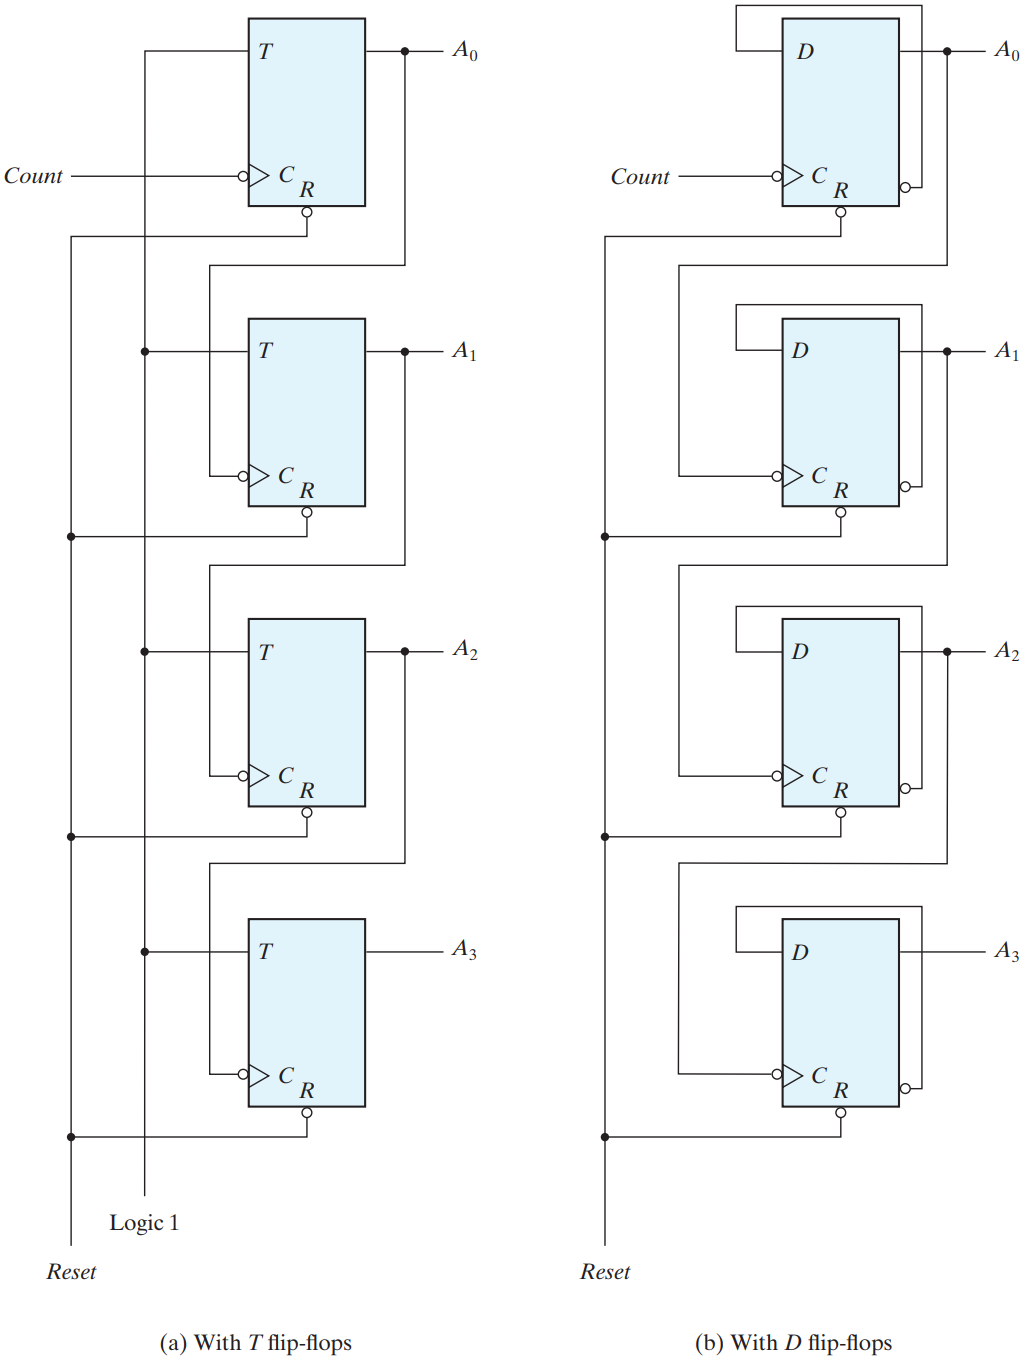
\includegraphics[width=\linewidth]{img/fig-6.8.png}
  \caption{Four-bit binary ripple counter}
  \label{fig:6.8}
\end{figure}

\noindent To understand the operation of the four-bit binary ripple counter, refer to the first nine binary numbers listed in Table 6.4. The count starts with binary 0 and increments by 1 with each count pulse input. The count starts with binary 0 and increments by 1 with each count pulse input. After the count of 15, the counter goes back to 0 to repeat the count

\begin{figure}[H]
  \centering
  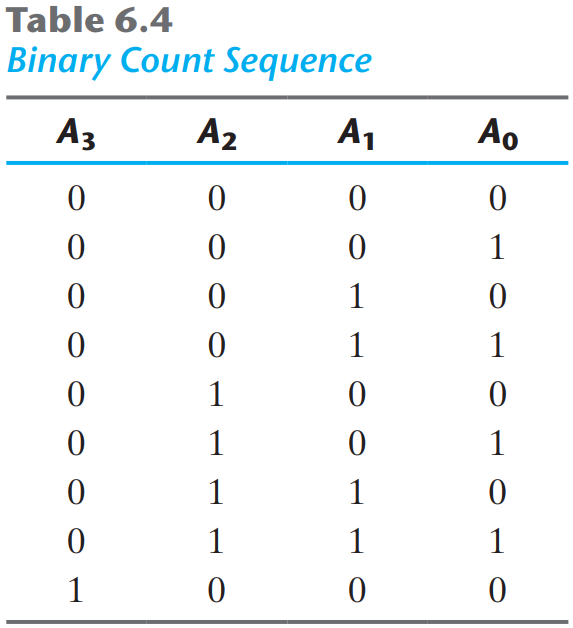
\includegraphics[width=.5\linewidth]{img/table-6.4.png}
  \label{table:6.4}
\end{figure}

A binary counter with a reverse count is called a \textit{binary countdown counter}. In a countdown counter, the binary count is decremented by 1 with every input count pulse. The count of a four-bit countdown counter starts from binary 15 and continues to binary counts 14, 13, 12, . . . , 0 and then back to 15.

\newpage

\subsection{BCD Ripple Counter}
\label{subsec:bcd-ripple-counter}

A decimal counter follows a sequence of 10 states and returns to 0 after the count of 9. If the BCD code is used, the sequence of states is as shown in the state diagram of Fig. 9.

\begin{figure}[H]
  \centering
  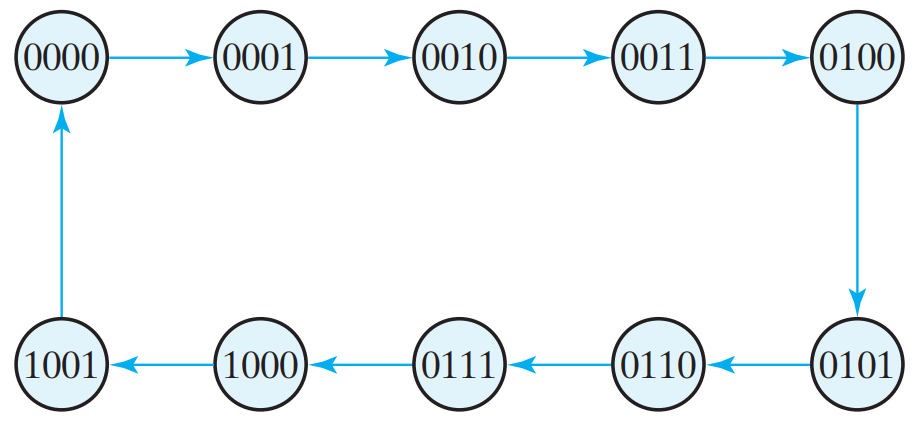
\includegraphics[width=\linewidth]{img/fig-6.9.png}
  \caption{State diagram of a decimal BCD counter}
  \label{fig:6.9}
\end{figure}

\noindent The logic diagram of a BCD ripple counter using JK flip-flops is shown in Fig. 10.

\begin{figure}[H]
  \centering
  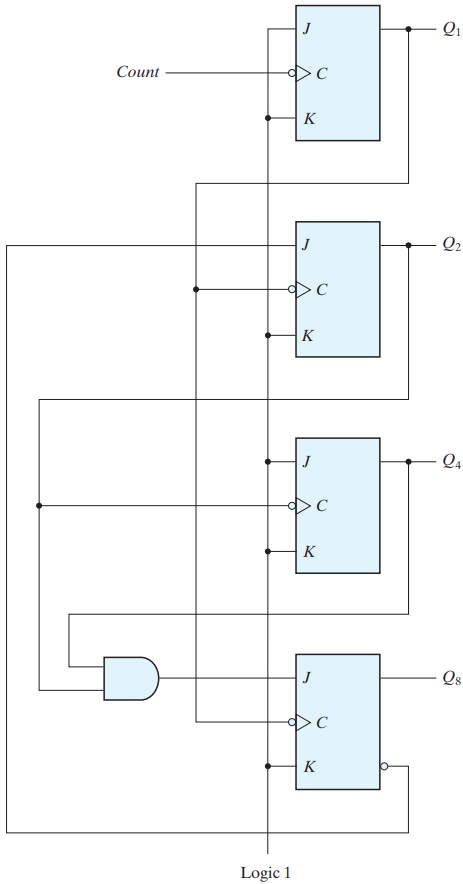
\includegraphics[width=.9\linewidth]{img/fig-6.10.png}
  \caption{BCD ripple counter}
  \label{fig:6.10}
\end{figure}

A ripple counter is an asynchronous sequential circuit. Its state changes are not synchronized to a common clock. Signals that affect the flip-flop transition depend on the way they change from 1 to 0.

The BCD counter of Fig. 10 is a \textit{decade counter}, since it counts from 0 to 9. To count from 0 to 999, we need a three-decade counter. A three-decade counter is shown in Fig. 11. 

\begin{figure}[H]
  \centering
  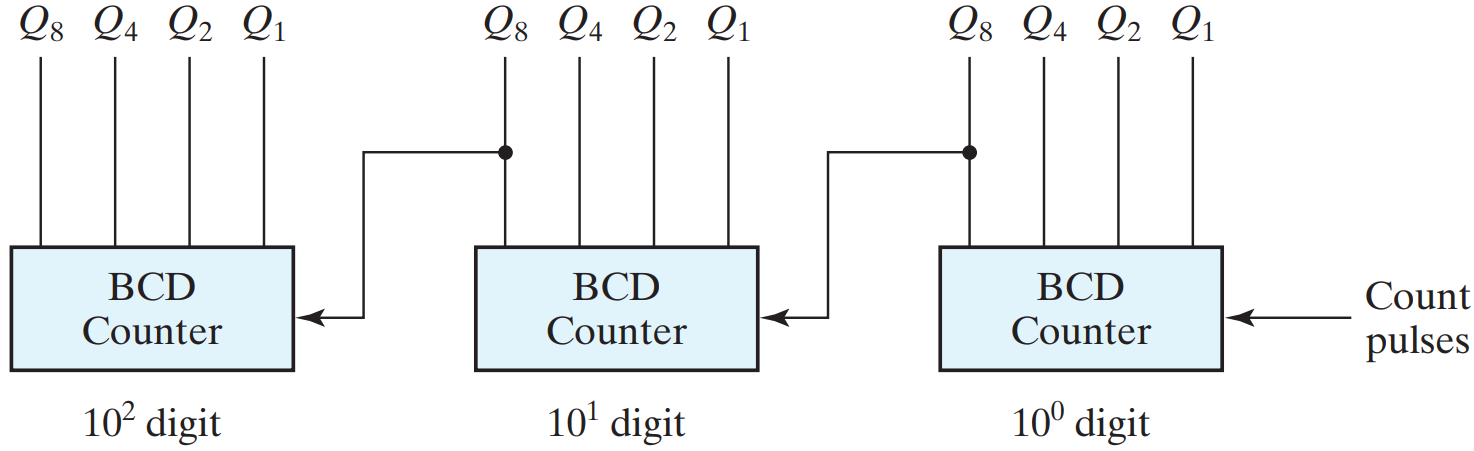
\includegraphics[width=\linewidth]{img/fig-6.11.png}
  \caption{BCD ripple counter}
  \label{fig:6.11}
\end{figure}


\section{Synchronous Counters}
\label{sec:synchronous-counters}

\textit{Synchronous counters} are different from ripple counters in that clock pulses are applied to the inputs of all flip-flops.

\subsection{Binary Counter}
\label{subsec:binary-counter}

In a synchronous binary counter, the flip-flop in the least significant position is complemented with every pulse. A \textit{flip-flop in any other position is complemented when all the bits in the lower significant positions are equal to 1}. 

\begin{figure}[H]
  \centering
  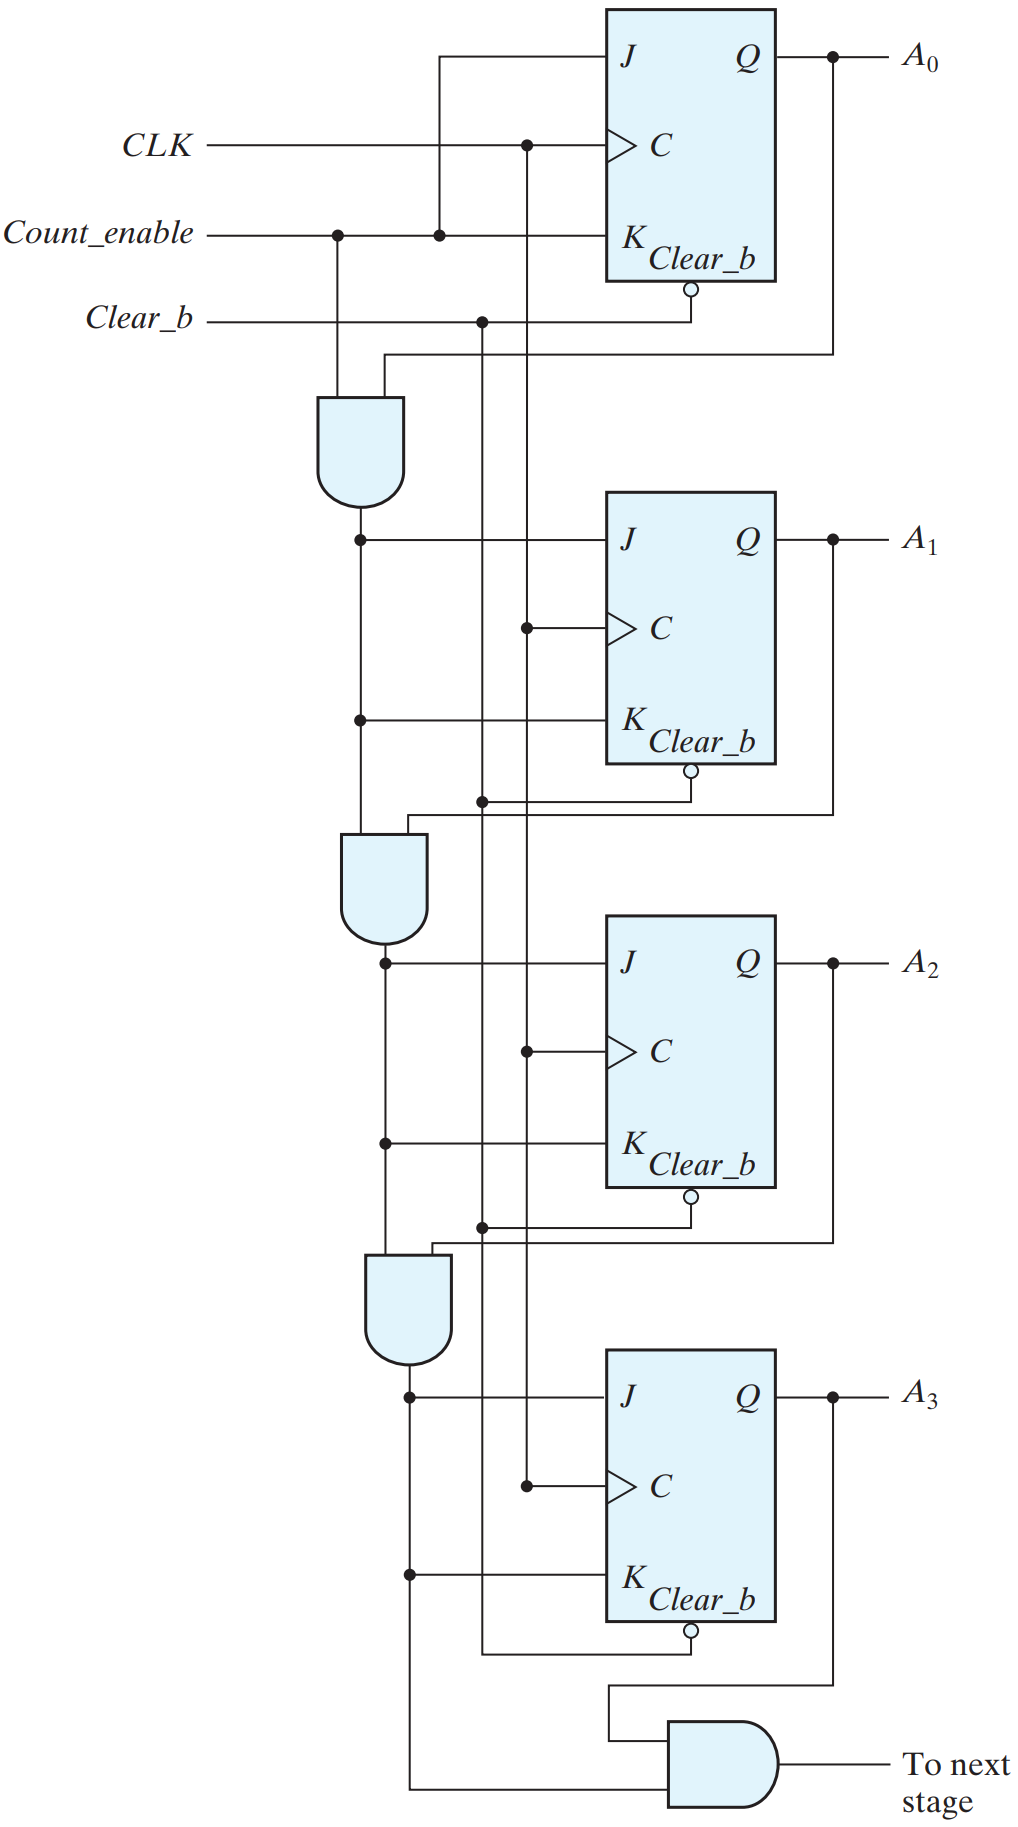
\includegraphics[width=.7\linewidth]{img/fig-6.12.png}
  \caption{Four-bit synchronous binary counter}
  \label{fig:6.12}
\end{figure}

\subsection{Up–Down Binary Counter}
\label{subsec:up-down-binary-counter}

A synchronous countdown binary counter goes through the binary states in reverse order, from 1111 down to 0000 and back to 1111 to repeat the count.

The bit in the least significant position is complemented with each pulse. \textit{A bit in any other position is complemented if all lower significant bits are equal to 0}.

A countdown binary counter can be constructed as shown in Fig. 12, except that the inputs to the AND gates must come from the complemented outputs, instead of the normal outputs, of the previous flip-flops. The two operations can be combined in one circuit to form a counter capable of counting either up or down. The circuit of an up–down binary counter using T flip-flops is shown in Fig. 13.

\begin{figure}[H]
  \centering
  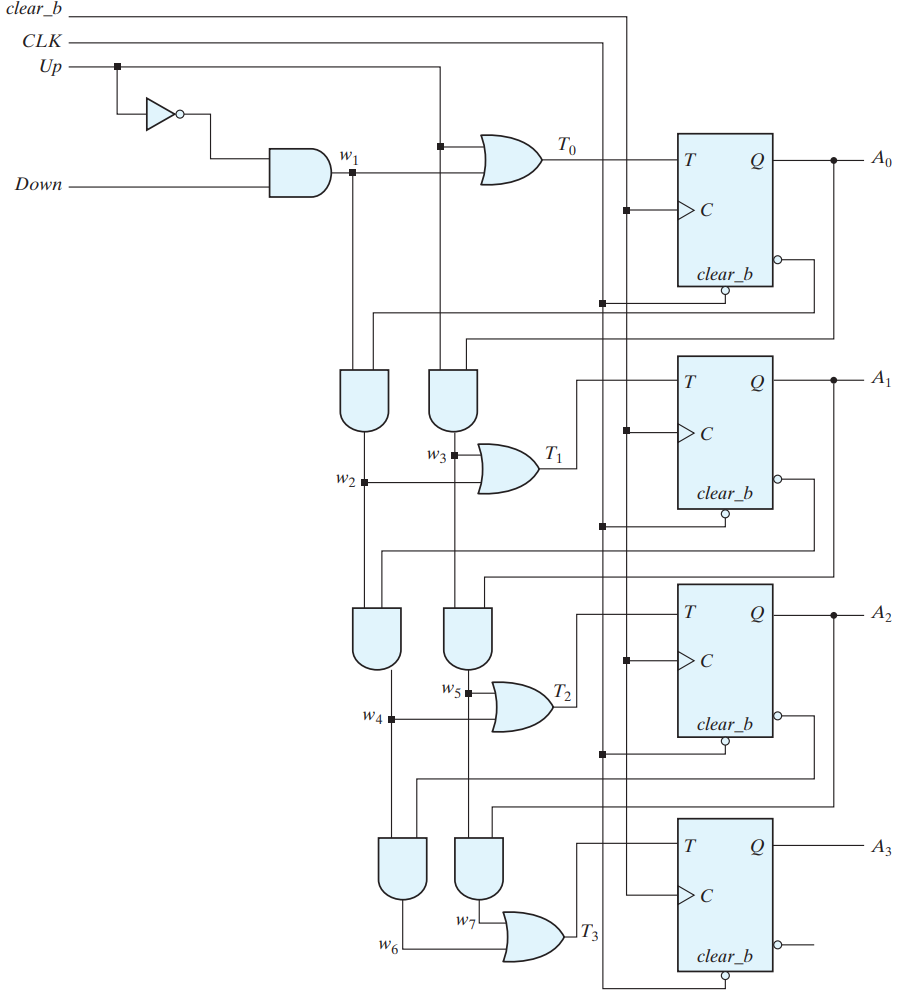
\includegraphics[width=\linewidth]{img/fig-6.13.png}
  \caption{Four-bit up–down binary counter}
  \label{fig:6.13}
\end{figure}

\subsection{BCD Counter}
\label{subsec:bcd-counter}

A BCD counter counts in binary-coded decimal from 0000 to 1001 and back to 0000. The state table of a BCD counter is listed in Table 6.5.

\begin{figure}[H]
  \centering
  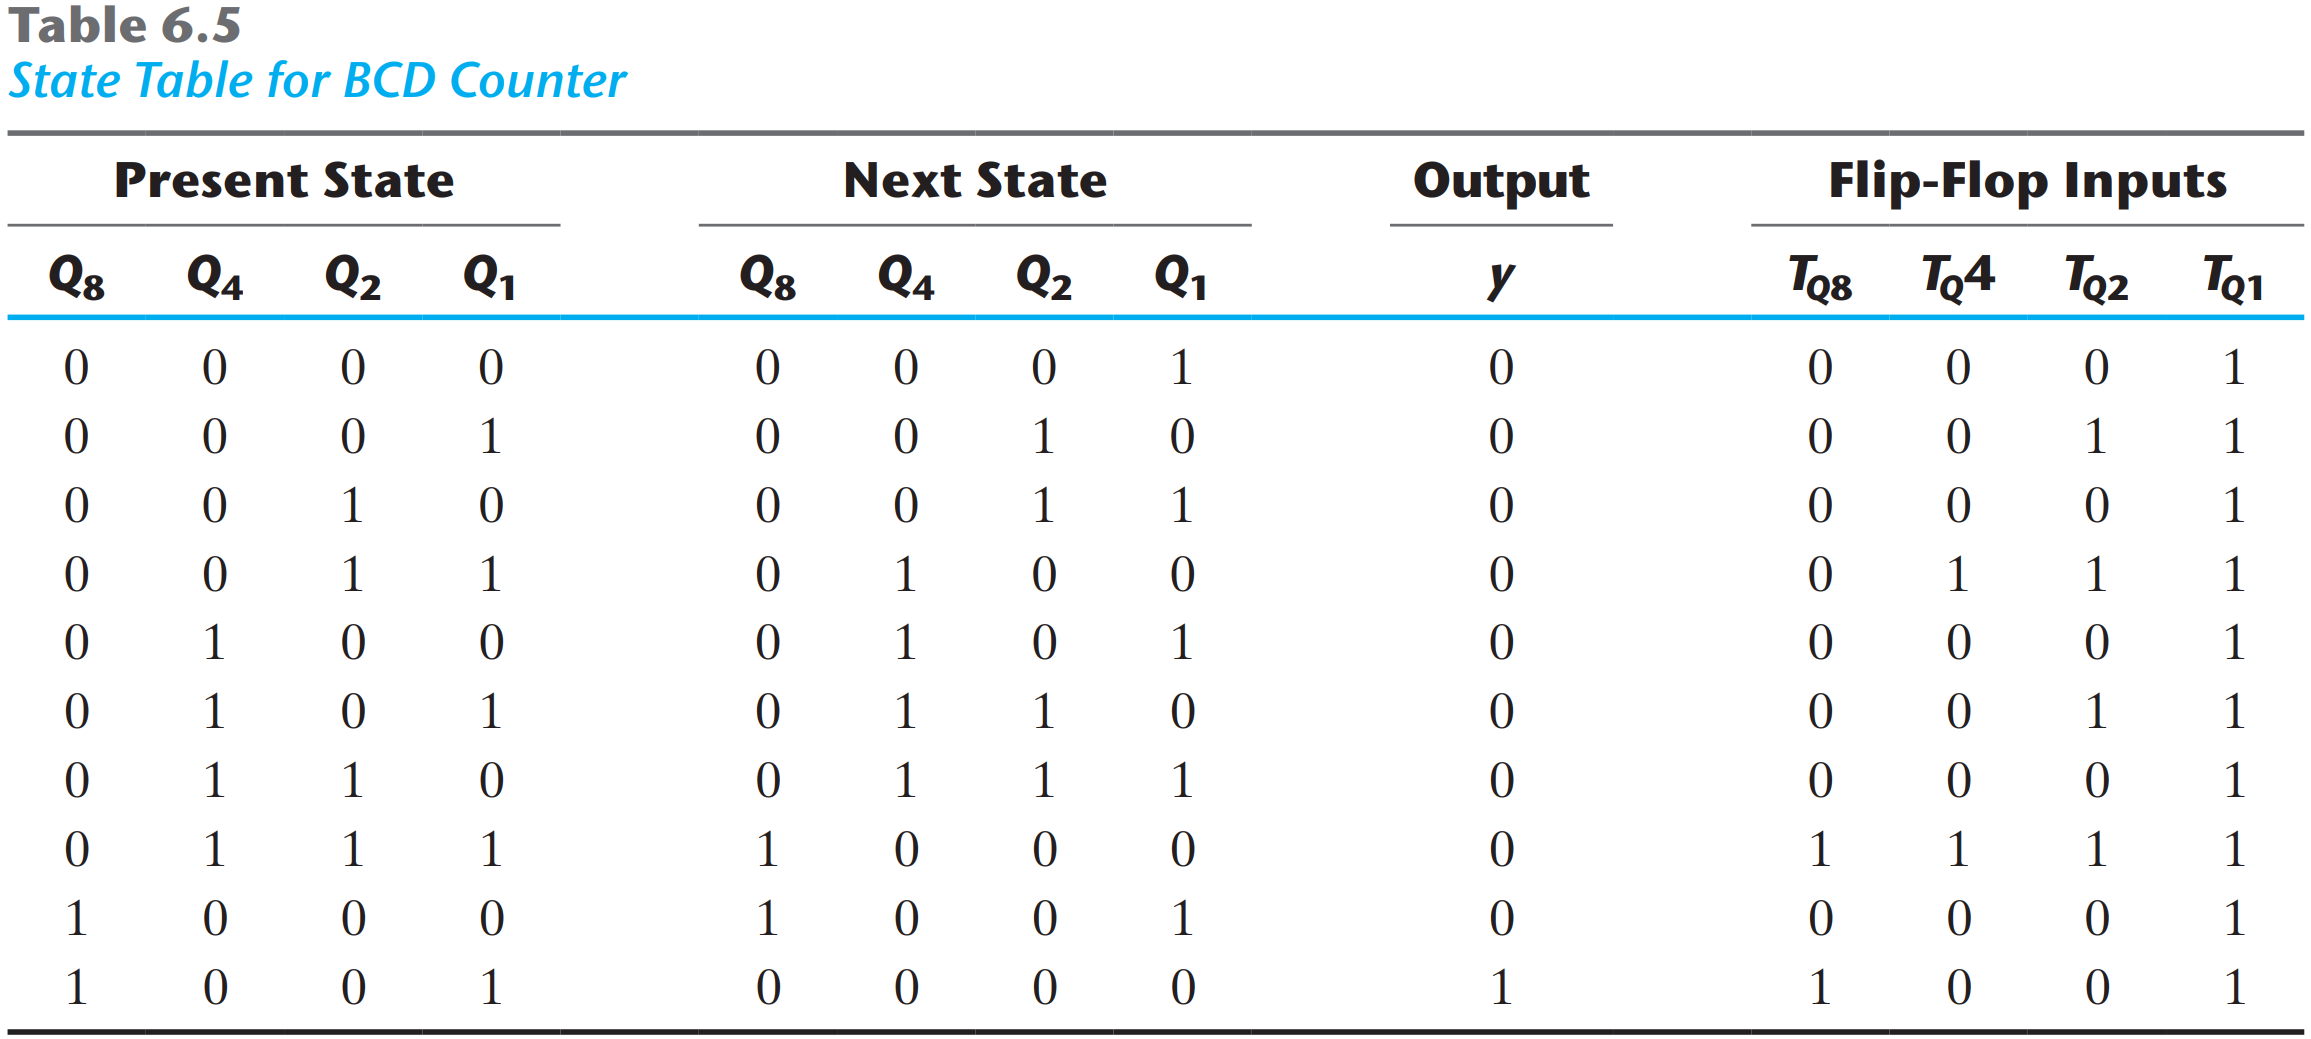
\includegraphics[width=.85\linewidth]{img/table-6.5.png}
  \label{table:6.5}
\end{figure}

The flip-flop input equations can be simplified:
\begin{align*}
  T_{Q_1} &= 1\\
  T_{Q_2} &= Q_8'Q_1\\
  T_{Q_4} &= Q_2Q_1\\
  T_{Q_8} &= Q_8Q_1 + Q_4Q_2Q_1\\
  y &= Q_8Q_1
\end{align*}
The circuit can easily be drawn with four $T$ flip-flops, five AND gates, and one OR gate.

\subsection{Binary Counter with Parallel Load}
\label{subsec:bin-counter-with-parallel-load}

Figure 14 shows the top-level block diagram symbol and the logic diagram of a four-bit register that has a parallel load capability and can operate as a binary counter.

\begin{figure}[H]
  \centering
  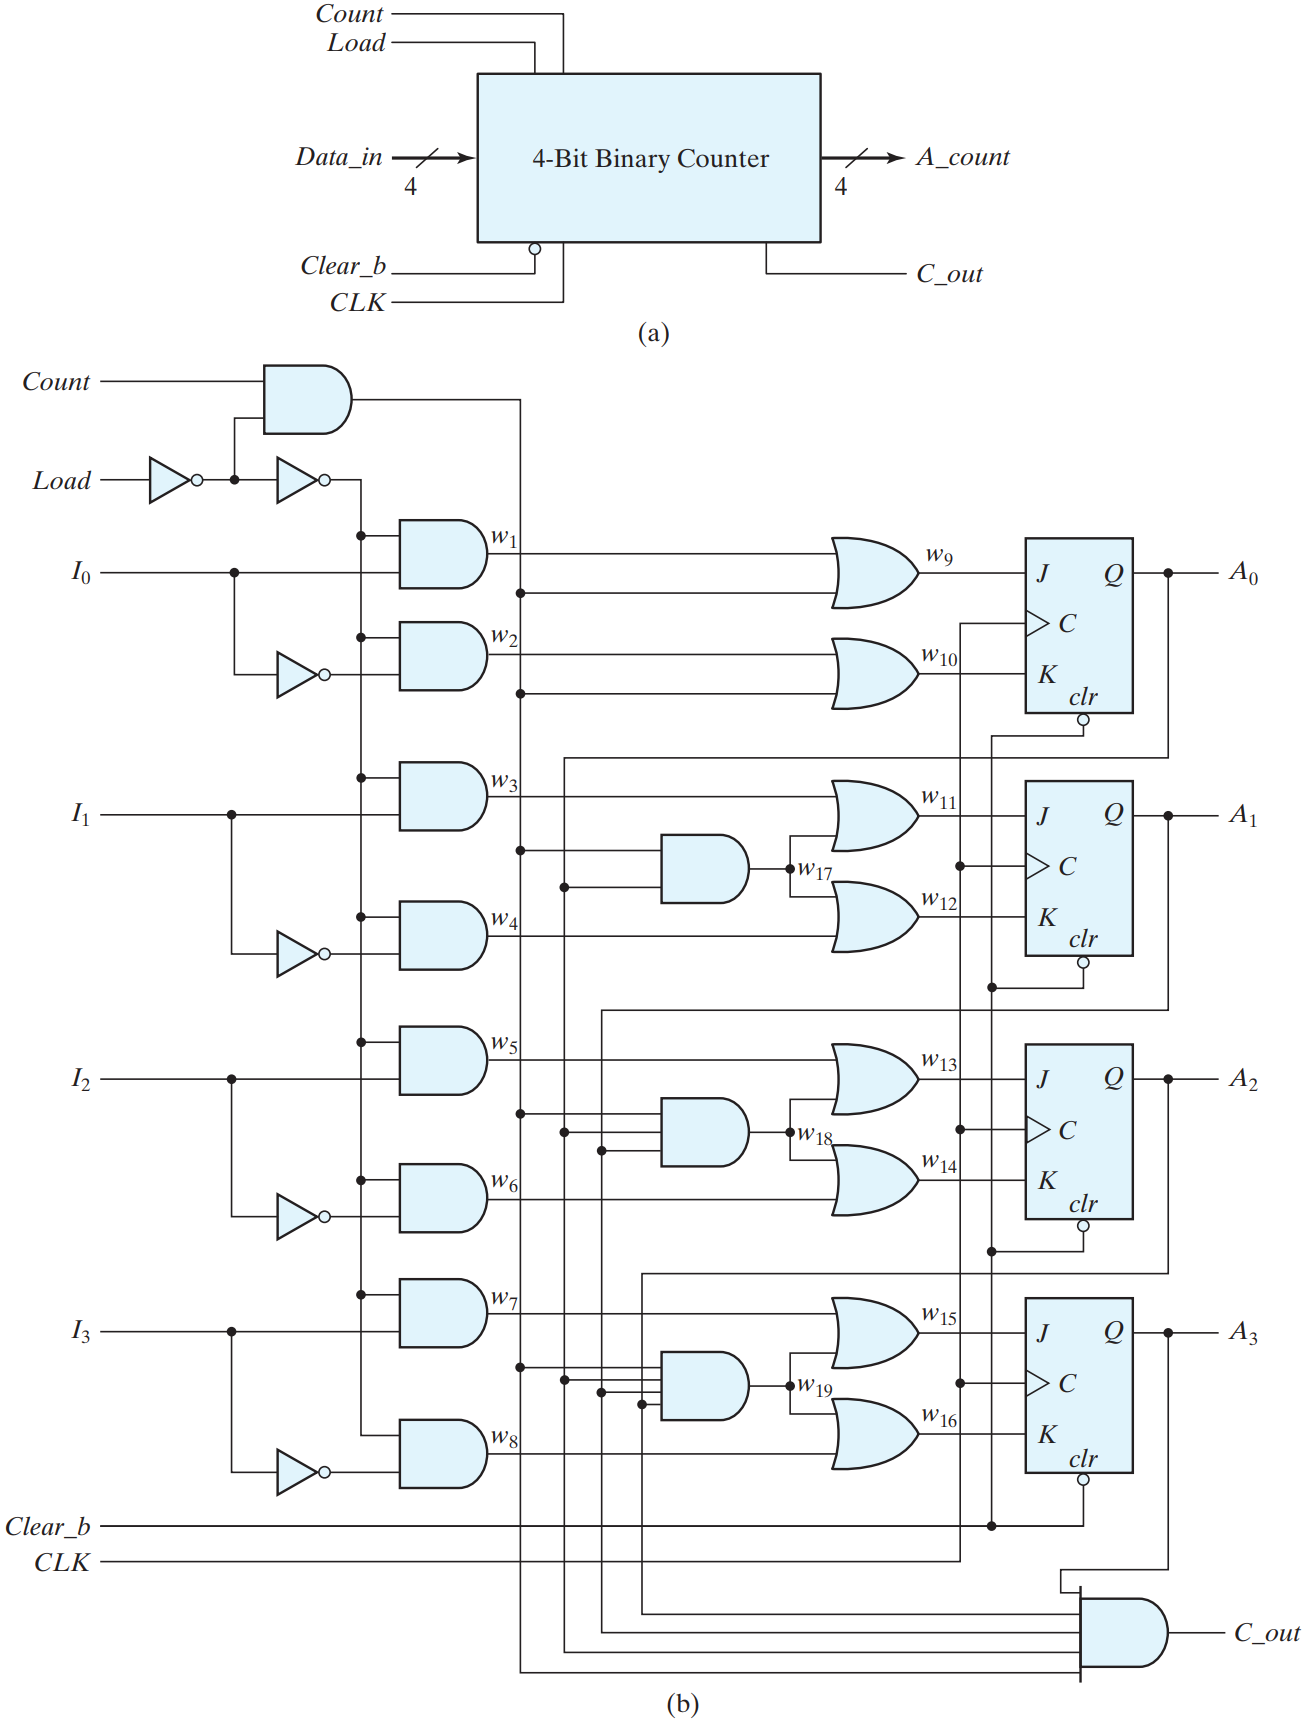
\includegraphics[width=\linewidth]{img/fig-6.14.png}
  \caption{Four-bit binary counter with parallel load}
  \label{fig:6.14}
\end{figure}

\noindent The operation of the counter is summarized in Table 6.6.

\begin{figure}[H]
  \centering
  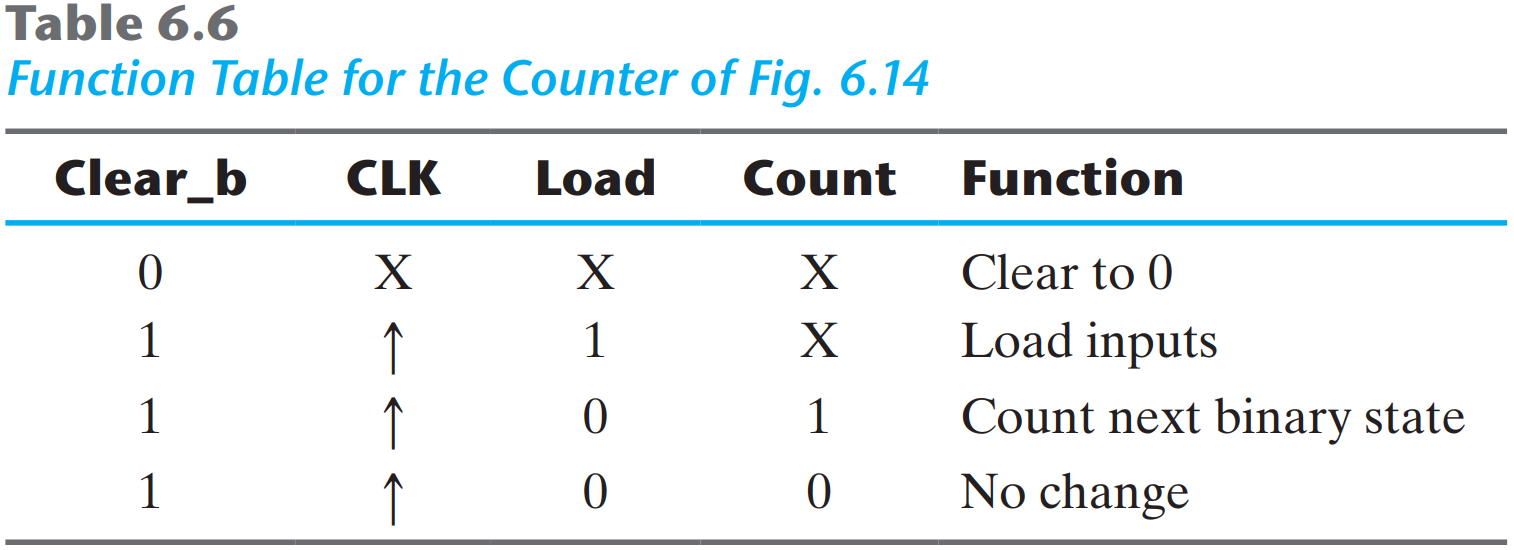
\includegraphics[width=\linewidth]{img/table-6.6.png}
  \label{table:6.6}
\end{figure}

\newpage

Figure 15 shows two ways in which a counter with a parallel load is used to generate the BCD count.
\begin{figure}[H]
  \centering
  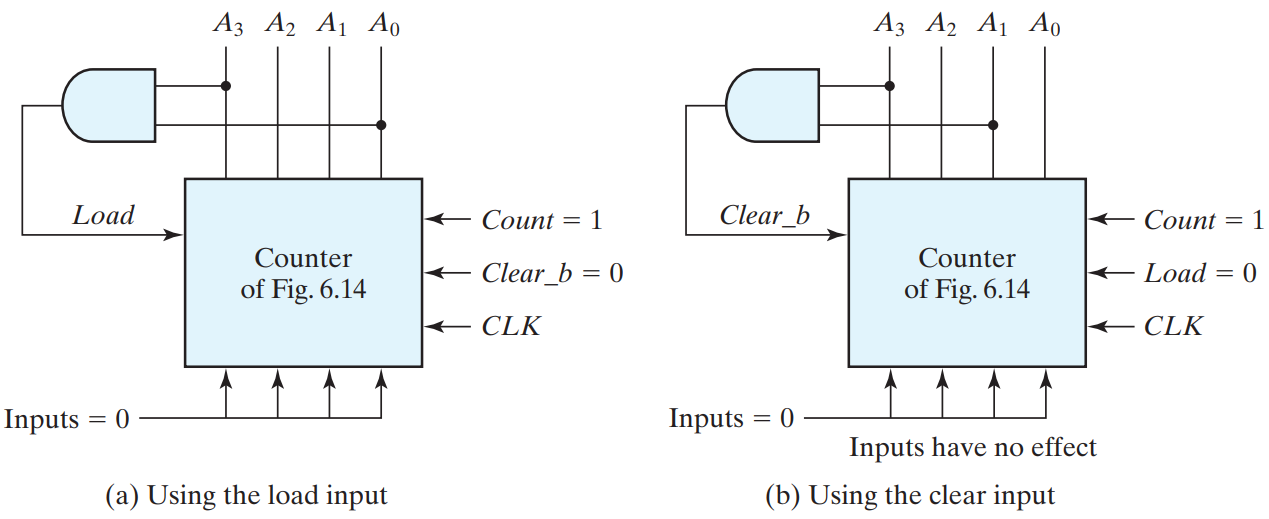
\includegraphics[width=\linewidth]{img/fig-6.15.png}
  \caption{Two ways to achieve a BCD counter using a counter with parallel load}
  \label{fig:6.15}
\end{figure}



\section{Other Counters}
\label{sec:other-counter}

\subsection{Counter with Unused States}
\label{subsec:counter-with-unused-states}

A circuit with $n$ flip-flops has $2^n$ binary states. However, sometimes one may have unused, or leftover states. In the end, we need to consider these states.

For example, condsider the following state table and diagram for a counter that repeatedly counts from 0 (000) to 5 (101). What should we put in the table for the two unused states.
\begin{figure}[H]
  \centering
  \begin{minipage}{0.49\linewidth}
      \centering
      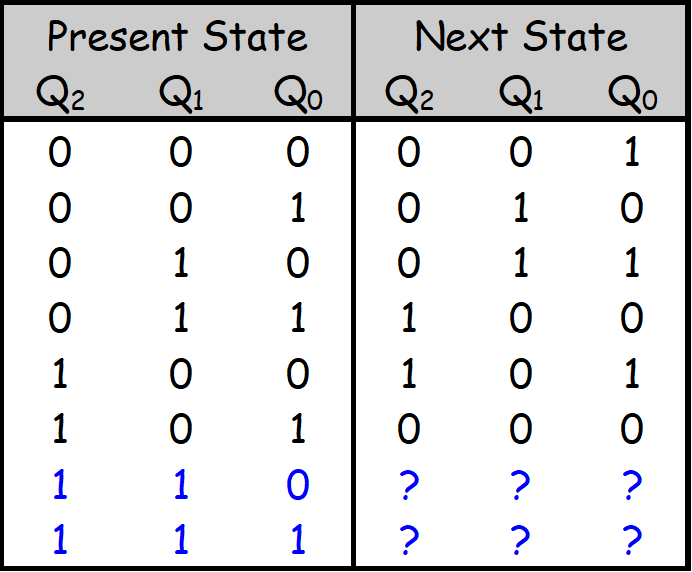
\includegraphics[width=\linewidth]{img/unused-state-table.png}
      \label{fig:unused-state-table}
  \end{minipage}\hfill
  \begin{minipage}{0.49\linewidth}
      \centering
      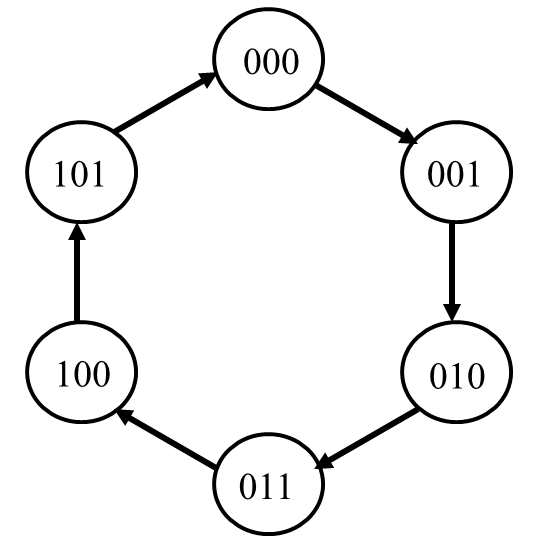
\includegraphics[width=\linewidth]{img/unused-state-diagram.png}
      \label{fig:unused-state-diagram.png}
  \end{minipage}
\end{figure}

To get the simplest possible circuit, you can fill in don't cares for the next states. This will also result in don't cares for the flip-flop inputs, which can simplify the hardware. If the circuit ``somehow'' ends up in one of the unused states (110 or 111), its behavior will depend on exactly what the don't cares were filled in with.

To get the safest possible circuit, you can explicitly fill in next states for the unused states 110 and 111. This guarantees that even if the circuit somehow enters an unused state, it will eventually end up in a valid state. This is called a self-starting counter.

\vspace*{\fill}
\columnbreak

\begin{figure}[H]
  \centering
  \begin{minipage}{0.49\linewidth}
    \centering
    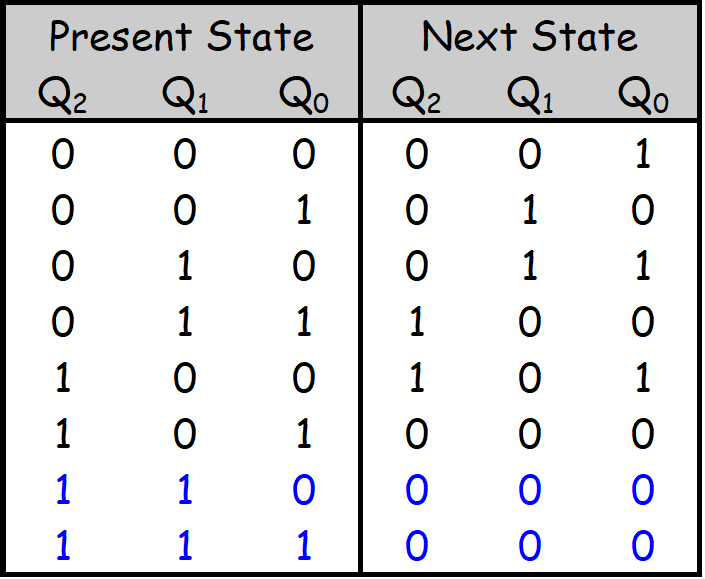
\includegraphics[width=\linewidth]{img/self-starting-counter-table.png}
    \label{fig:self-starting-counter-table.png}
  \end{minipage}\hfill
  \begin{minipage}{0.49\linewidth}
    \centering
    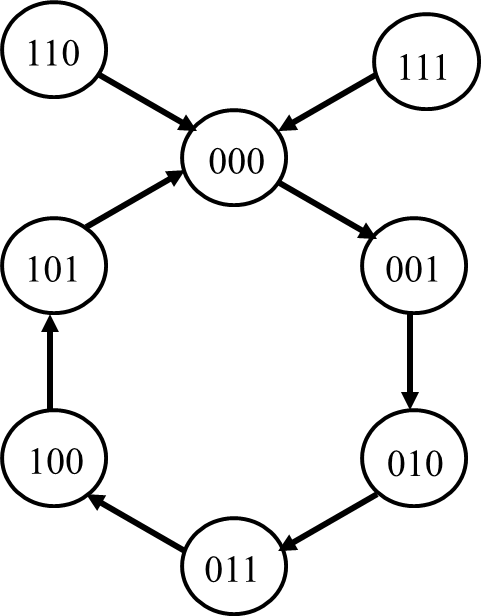
\includegraphics[width=\linewidth]{img/self-starting-counter-diagram.png}
    \label{fig:self-starting-counter-diagram.png.png}
  \end{minipage}
\end{figure}

\subsection{Ring Counter}
\label{subsec:ring-counter}

A \textit{ring counter} is a circular shift register with only one flip-flop being set at any particular time; all others are cleared.

The single bit is shifted from one flip-flop to the next to produce the 
sequence of timing signals. Figure 17(a) shows a four-bit shift register connected as a 8-4-2-1 ring counter. For an alternative design, the timing signals can be generated by a two-bit counter that goes through four distinct states. The decoder shown in Fig. 17(c) decodes the four states of the counter and generates the required sequence of timing signals.


To generate $2^n$ timing signals, we need either a shift register with $2^n$ flip-flops or an $n$-bit binary counter together with an $n$-to-$2^n$-line decoder.

\subsection{Johnson Counter}
\label{subsec:johnson-counter}

A $k$-bit ring counter circulates a single bit among the flip-flops to provide $k$ distinguishable states. The number of states can be doubled if the shift register is connected as a \textit{switch-tail ring counter}. Figure 18(a) shows such a shift register.

Starting from a cleared state, the switch-tail ring counter goes through a sequence of eight states, as listed in Fig. 18(b). In general, a $k$-bit switch-tail ring counter will go through a sequence of $2k$ states.

\vspace*{\fill}
\columnbreak

\setcounter{figure}{16}

\begin{figure}[H]
  \centering
  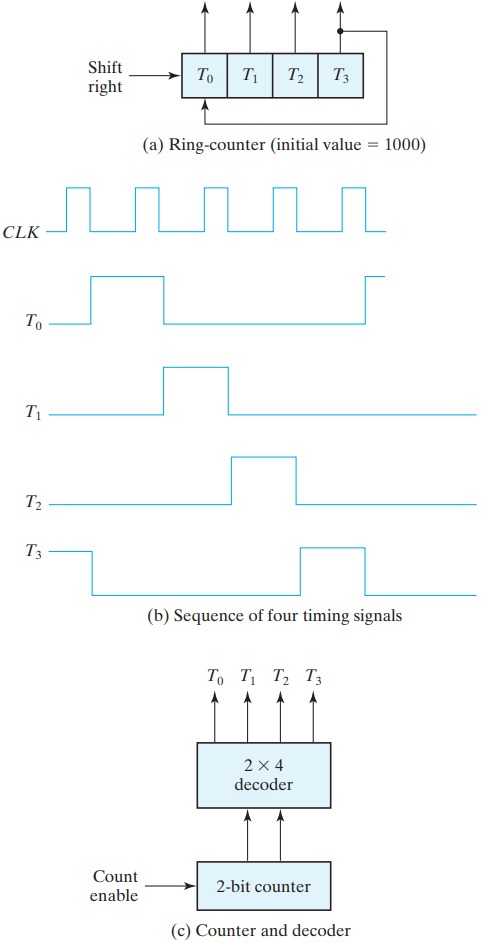
\includegraphics[width=.9\linewidth]{img/fig-6.17.png}
  \caption{Generation of timing signals}
  \label{fig:6.17}
\end{figure}

\begin{figure}[H]
  \centering
  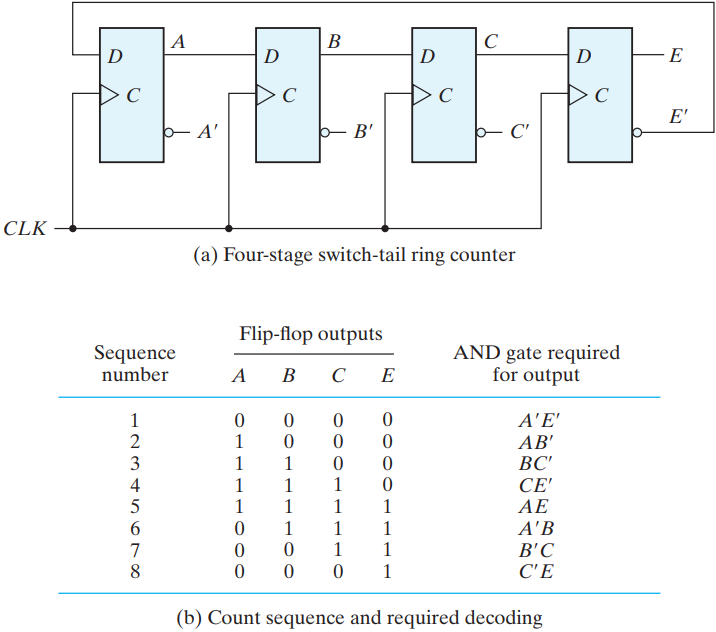
\includegraphics[width=.9\linewidth]{img/fig-6.18.png}
  \caption{Construction of a Johnson counter}
  \label{fig:6.18}
\end{figure}


\section{Summary}

\subsection{Register}

\begin{itemize}
  \item A register is a special sequential circuit that stores multiple bits of data. Several variations are possible:
    \begin{itemize}
      \item Parallel loading to store data into the register.
      \item Shifting the register contents either left or right.
      \item Counters are considered a type of register too!
    \end{itemize}
  
  \item One application of shift registers is converting between serial and parallel data.
  \item Registers are a central part of modern processors, as we will see in coming weeks.
\end{itemize}

\subsection{Counters}

\begin{itemize}
  \item Counters serve many purposes in sequential logic design.
  \item There are lots of variations on the basic counter.
    \begin{itemize}
      \item Some can increment or decrement.
      \item An enable signal can be added.
      \item The counter's value may be explicitly set.
    \end{itemize}
  
  \item There are also several ways to make counters.
  \begin{itemize}
    \item You can follow the sequential design principles from last week to build counters from scratch.
    \item You could also modify or combine existing counter devices.
  \end{itemize}  
\end{itemize}

\end{multicols*}

\end{document}
